% !TeX spellcheck = en_GB
% encoding: utf8
% !TEX encoding = utf8
% !TEX program = pdflatex
% !BIB program = biber

\documentclass[11pt,oneside,a4paper]{report}

\usepackage[utf8]{inputenc}
\usepackage[T1]{fontenc}
\usepackage[colorlinks]{hyperref}
\usepackage[left=2.5cm, right=2.5cm, top=2.5cm, bottom=2.5cm]{geometry}
\usepackage{float}
\usepackage{subcaption}
\usepackage{mathtools}
\usepackage{color}
\usepackage{listings}
\usepackage{xcolor}
\usepackage[backend=biber,maxnames=10,style=numeric,sorting=nty,abbreviate=false,giveninits=true,language=english]{biblatex}

\addbibresource{../meros.bib}

%\newcommand{\twc}[1]{\textcolor{red}{\textbf{TW}: #1}}
\newcommand{\Fig}[1]{Fig.~\ref{#1}}

\definecolor{amber}{rgb}{1.0, 0.49, 0.0}
\newcommand{\twci}[1]{
	\textcolor{amber}{TW: #1}}

% encoding: utf8
%
% Stereotypes
%

% Lista powinna być zgodna z profilem w EA

\newcommand{\stActionConn}{<<Action>>}
\newcommand{\stCommChannel}{<<CommChannel>>}
\newcommand{\stComponContain}{<<ComponContain>>}
\newcommand{\stGpPackages}{<<GpPackages>>}
\newcommand{\stHardware}{<<Hardware>>}
\newcommand{\stLaunchFile}{<<LaunchFile>>}
\newcommand{\stMetaPackage}{<<MetaPackage>>}
\newcommand{\stMicroNode}{<<MicroNode>>}
\newcommand{\stNamespace}{<<Namespace>>}
\newcommand{\stNode}{<<Node>>}
\newcommand{\stPackage}{<<Package>>}
\newcommand{\stParameter}{<<Parameter>>}
\newcommand{\stRepository}{<<Repository>>}
\newcommand{\stRosCommCompon}{<<RosCommCompon>>}
\newcommand{\stRosConn}{<<RosConn>>}
\newcommand{\stRQtNode}{<<RQtNode>>}
\newcommand{\stRunSystemCompon}{<<RunSystemCompon>>}
\newcommand{\stServiceConn}{<<Service>>}
\newcommand{\stSourExeContain}{<<SourExeContain>>}
\newcommand{\stSystem}{<<System>>}
\newcommand{\stTerminal}{<<Terminal>>}
\newcommand{\stTopicConn}{<<Topic>>}
\newcommand{\stWorkspace}{<<Workspace>>}

\newcommand{\stblock}{<<block>>}






\lstdefinestyle{terminal}{
	backgroundcolor=\color{black},
	basicstyle=\ttfamily\color{green},
	frame=single,
	rulecolor=\color{gray},
}


\begin{document}
	
\title{MeROS: SysML-based Metamodel for ROS-related Systems - version 4.0.0 - reference manual}
\author{MeROS developers group - https://github.com/twiniars/MeROS \\ tomasz.winiarski@pw.edu.pl}
\date{\today}
\maketitle


\begin{abstract}
	The complexity of today's robot control systems implies difficulty in developing them efficiently and reliably. Systems engineering (SE) and frameworks come to help. The frameworks' metamodels are needed to support the standardisation and correctness of the created application models. MeROS is a~metamodel for ROS, which addresses the running system and developer workspace. An essential addition to the original ROS concepts is the grouping of these concepts, which provides an opportunity to illustrate the system's decomposition and varying degrees of detail in its presentation. The metamodel is derived from the requirements and verified on the practical examples. The matter is described in a~standardised way in SysML (Systems Modeling Language). Hence, common development tools that support SysML can help develop robot controllers in the spirit of SE.
\end{abstract}
	
	
	
	\maketitle
	
\chapter*{Experiments}

\begin{lstlisting}[style=terminal]
	$ git status
	On branch main
	nothing to commit, working tree clean
\end{lstlisting}

	
	
	
	
\chapter*{Important citation notice}

\textbf{If you are to use MeROS in your papers, please first cite the IEEE ACCESS  article~\cite{meros-access}, where the initial version of the MeROS is presented. You can also refer to MeROS project page \cite{meros-www} and mention the actual MeROS version you are using.} 
	
	
\chapter{MeROS application}
\label{ch:application}
	
	\twci{Do aktualizacji. Ma być przykład z turtlesimem. W tym przykładzie będzie omówienie jak on powstawał, w sensie dodatkowych zrzutów ekranu z retrospekcji działającego systemu ROS. Czyli pokazujemy jak za pomocą rosowych komend uzyskać informacje potrzebne do stworzenia modelu. Jest to bezcenne na ANRO i nie tylko.}
	

	
	This documentation presents key aspects of an exemplary system development process incorporating MeROS. The exemplary system was created within the AAL INCARE project to control the Rico assistive robot (modified TIAGo platform with controller based on ROS~1) to execute transportation attendance tasks (Fig.~\ref{fig:herbatka_u_winiara}).
	
	\begin{figure}[H]
		\centering
		\begin{center}
			{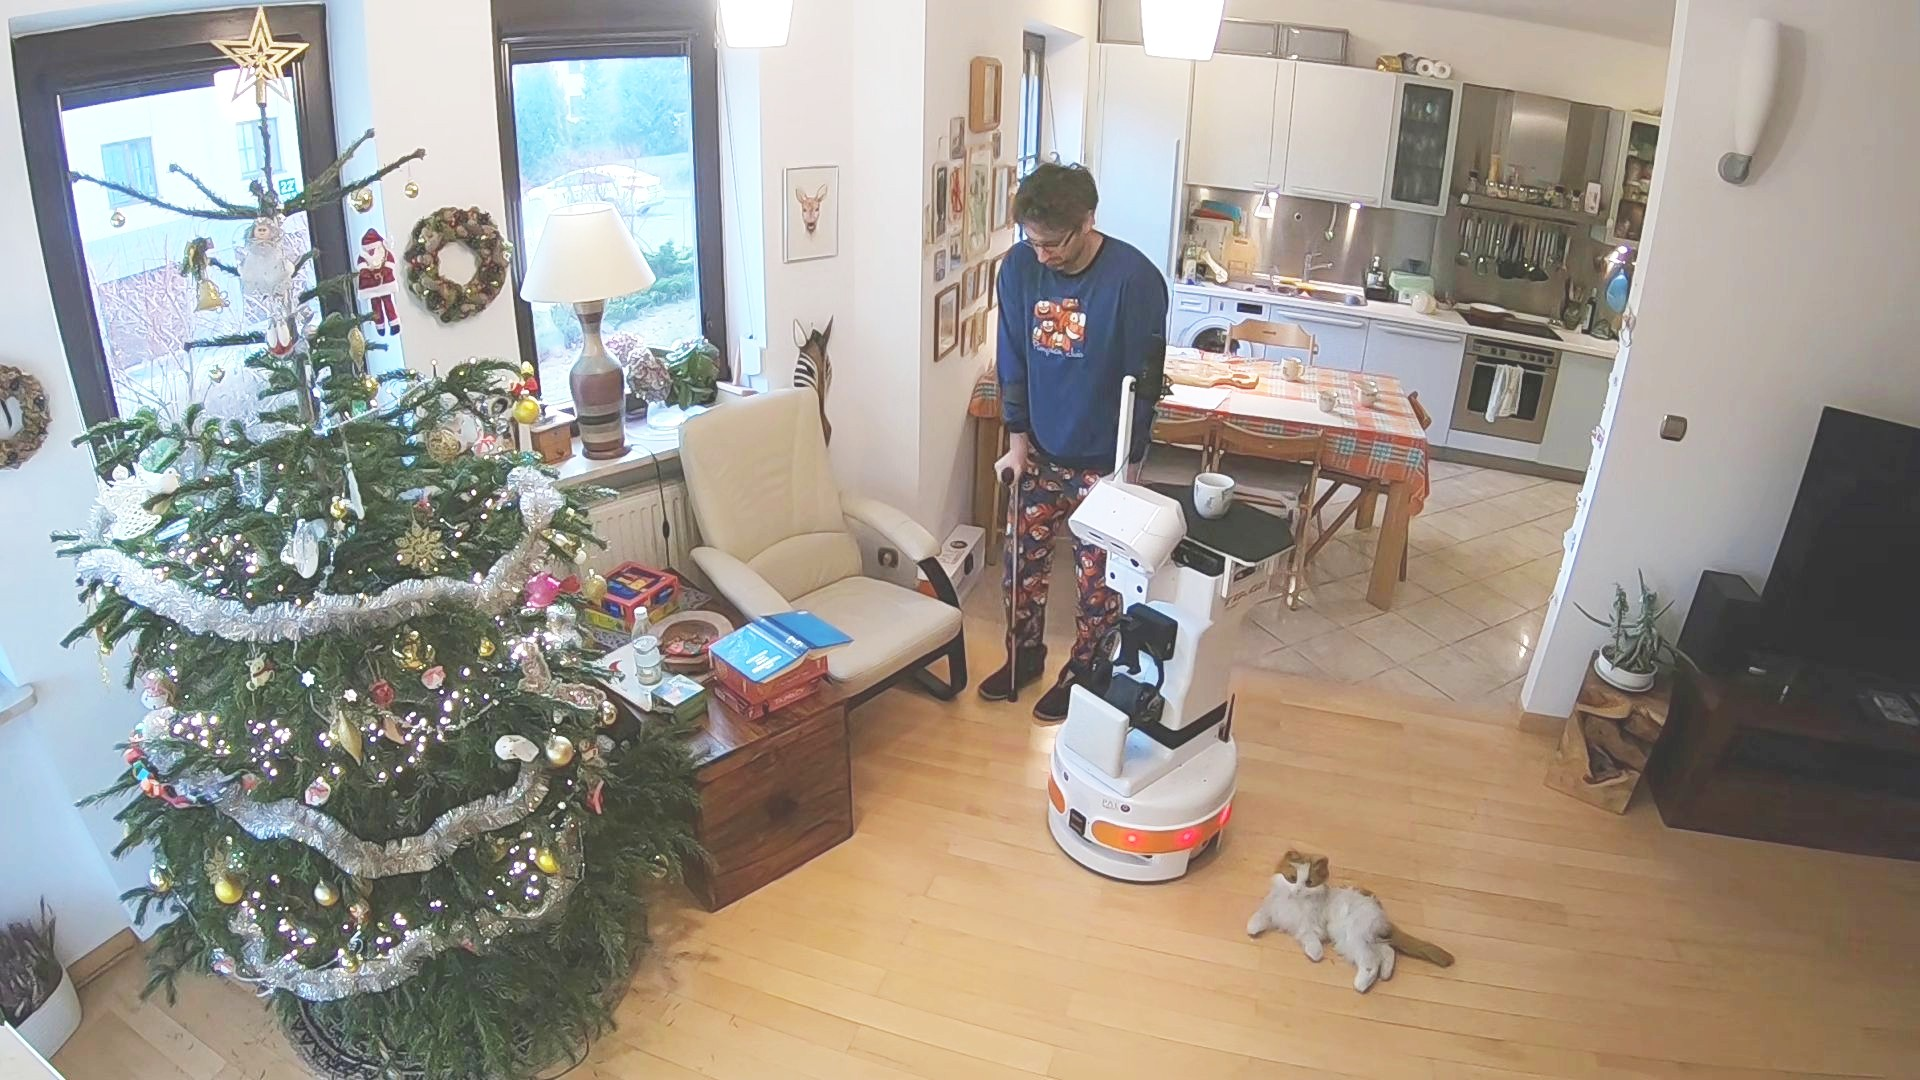
\includegraphics[width=\columnwidth]{img/herbatka_u_winiara.jpg}}
		\end{center}
		\caption{Transportation attendance by Rico robot \url{https://vimeo.com/670252925}} 
		\label{fig:herbatka_u_winiara}
	\end{figure}
	
	
	
	 The purpose of the following description is not to document the entire system but to illustrate, by example, representative aspects of the MeROS application.
	 
	\newpage
	The Rico \stSystem{} consists of two parts. Its \stWorkspace{} and a~number of \stRunSystemCompon{} (Fig.~\ref{fig:rico_system_bdd}).
	
	
	\begin{figure}[H] 
		\centering
		\begin{center}
			{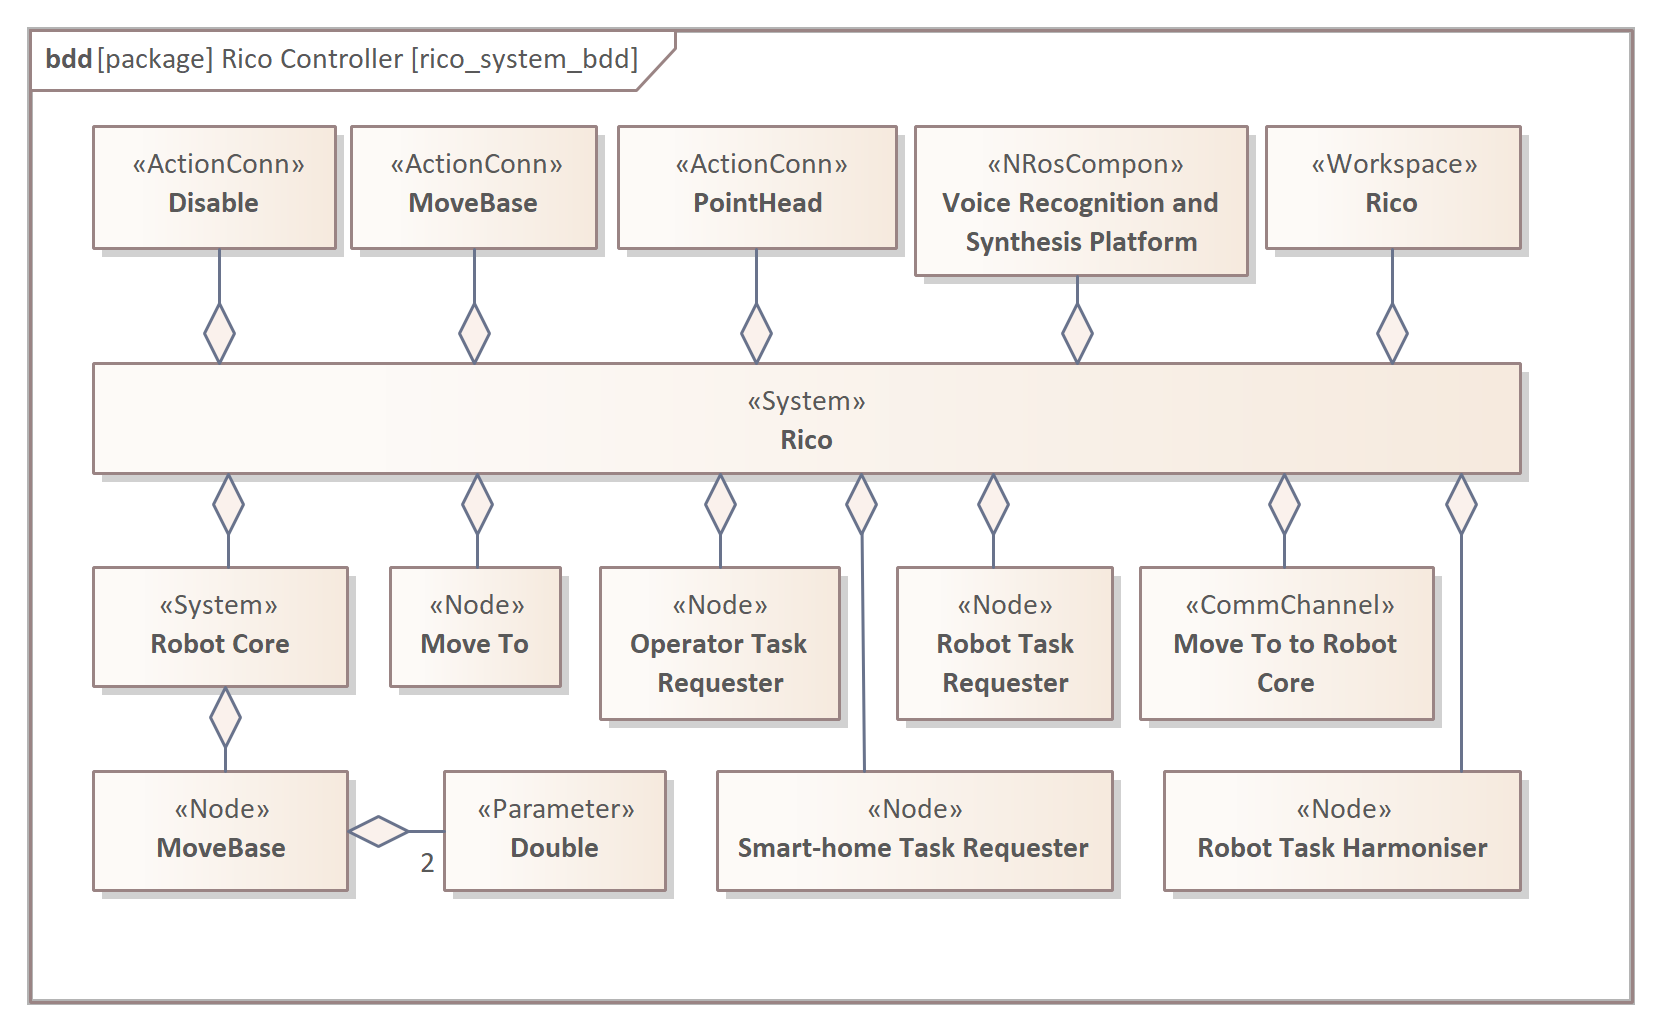
\includegraphics[scale=.9]{img/rico_pkg/rico_system_bdd.png}}
		\end{center}
		\caption{Rico \stSystem{} composition.} 
		\label{fig:rico_system_bdd}
	\end{figure}
	
	
	The fragment of the application scenario is conceptually presented in Fig.~\ref{fig:general_sd}.
	

	\begin{figure}[H] 
		\centering
		\begin{center}
			{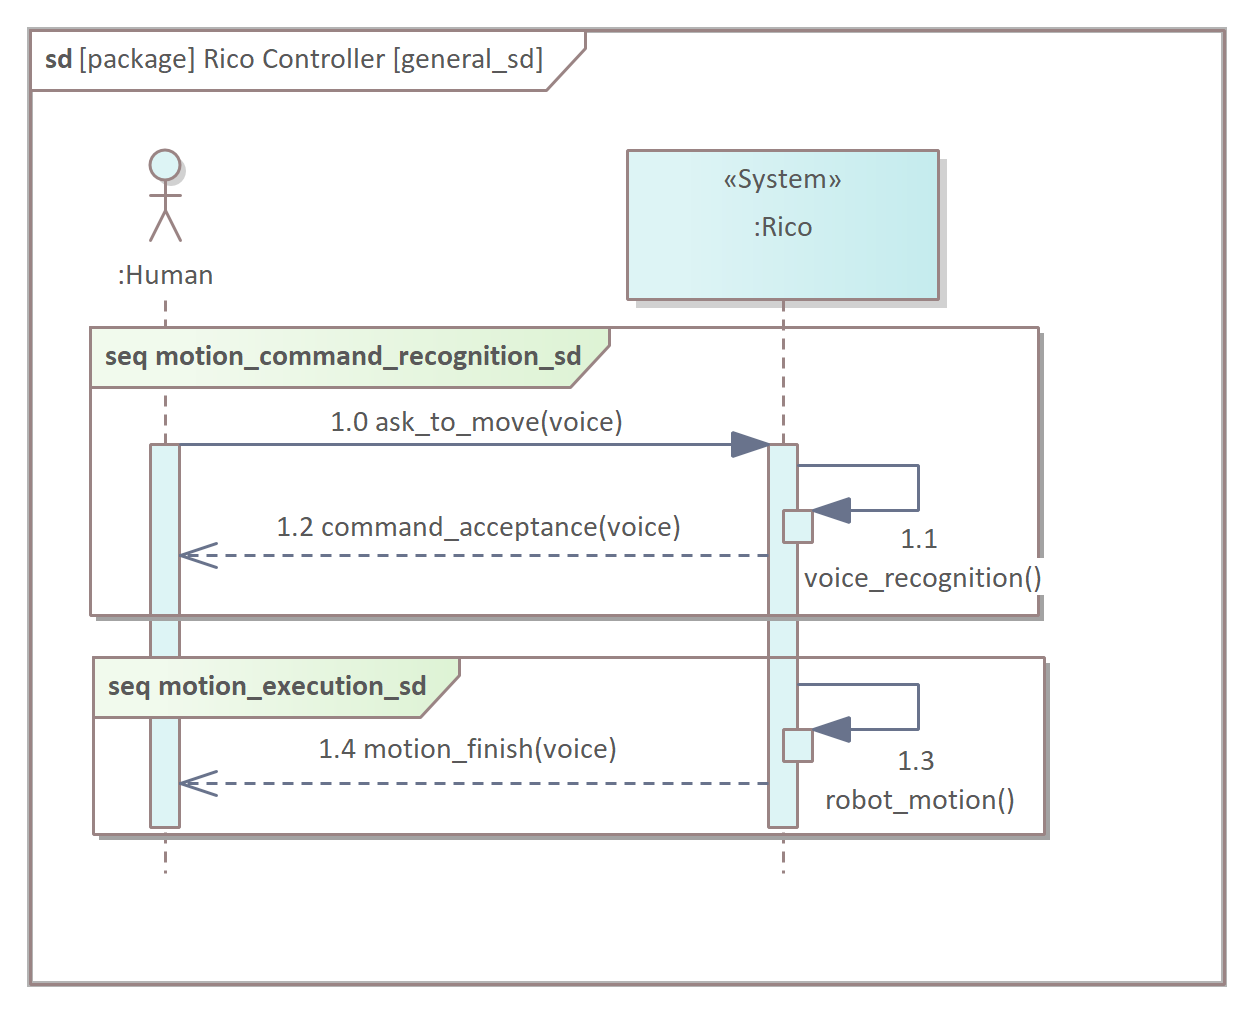
\includegraphics[scale=.9]{img/rico_pkg/general_sd.png}}
		\end{center}
		\caption{Concept scenario.} 
		\label{fig:general_sd}
	\end{figure}
	
	Here, the system (\stSystem{} \texttt{:Rico}) and its behaviour are formulated in a~general way. An actor (e.g. an elderly person) asks the robot to move. Then, the system recognises the voice command and vocally confirms the command's acceptance. Finally, the robot executes the motion and vocally informs that the motion is finished.
	In the following part of the description, the \stSystem{} \texttt{:Rico} and sequence diagram frame \texttt{motion execution} from Fig.~\ref{fig:general_sd} are presented in a~explicit way.
	
		The \stSystem{} \texttt{:Rico} structure is depicted in Fig.~\ref{fig:rico_system_ibd}. Here, and in the following diagrams, the \texttt{rosout} and \texttt{ROS master} \stNode{}s were omitted to make the diagrams more compact. Dedicated block is needed for \stCommChannel{} \texttt{:Move To to Robot Core}, because this \stCommChannel{} is specified in detail later on.
	
	\begin{figure}[H]
		\centering
		\begin{center}
			{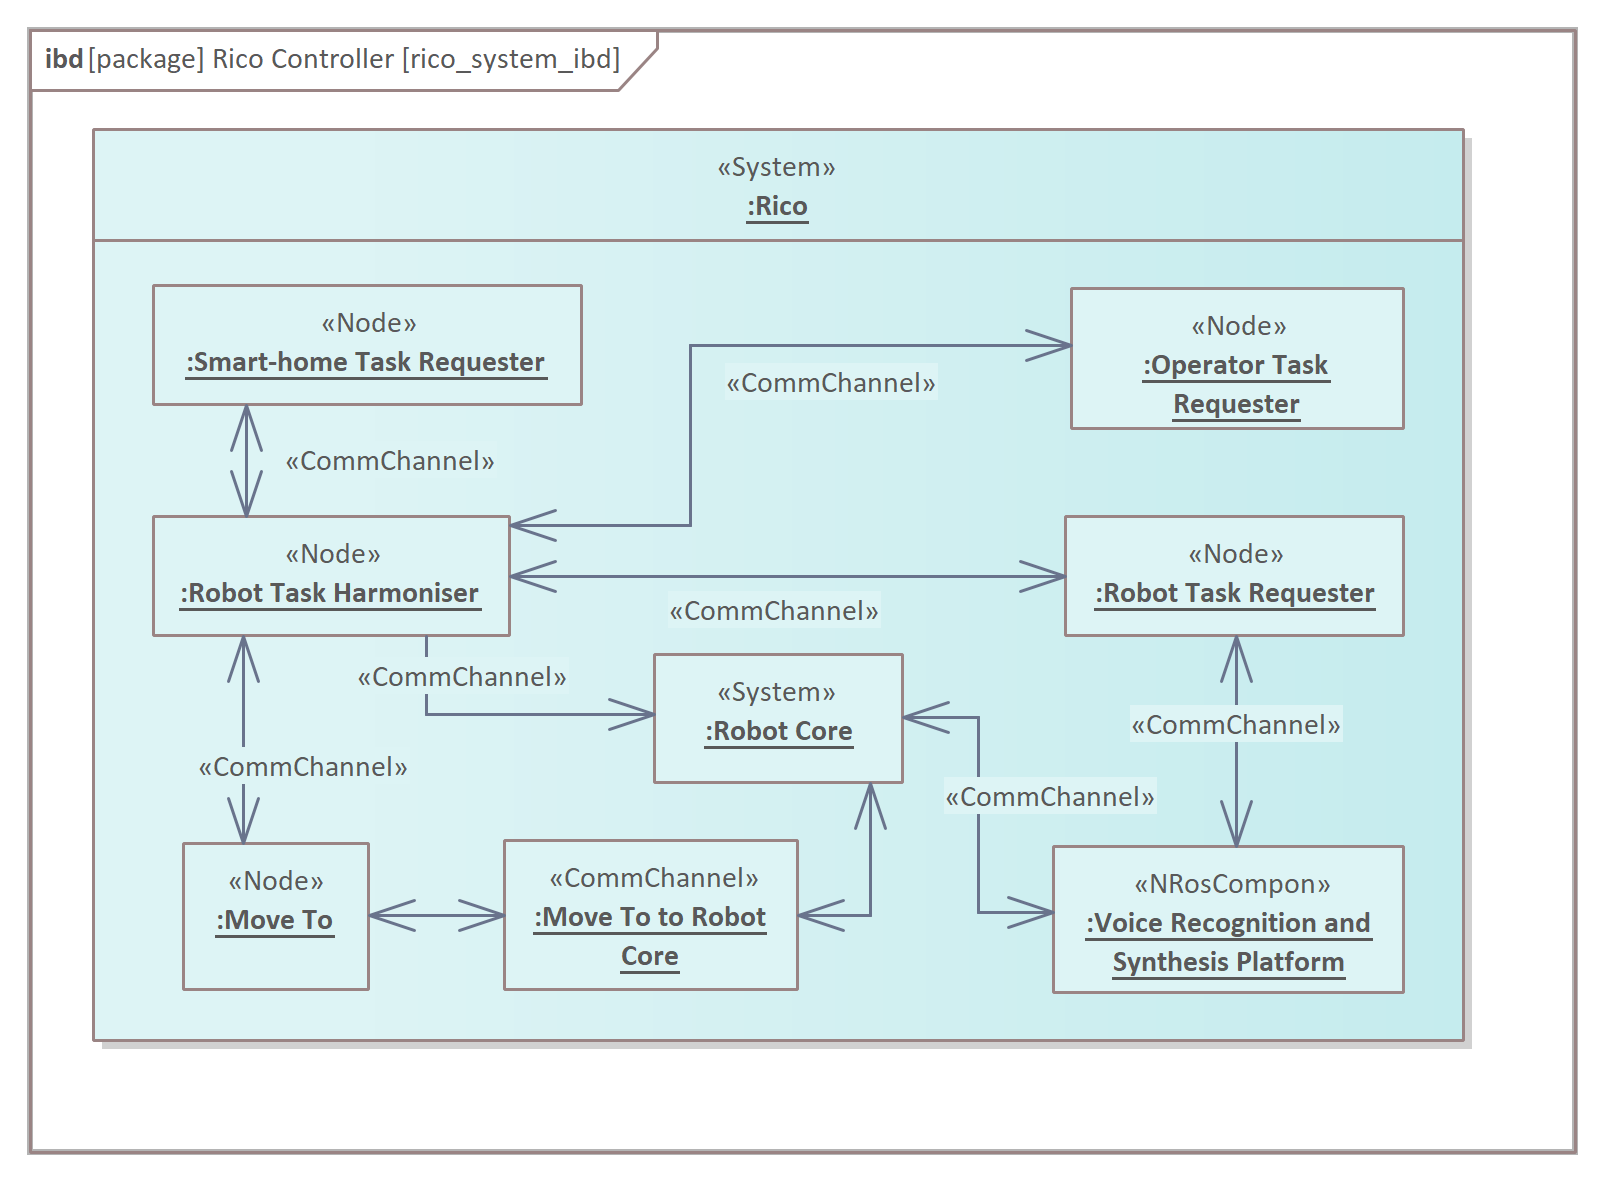
\includegraphics[scale=0.85]{img/rico_pkg/rico_system_ibd.png}}
		\end{center}
		\caption{Structure of \stSystem{}\texttt{:Rico}.} 
		\label{fig:rico_system_ibd}
	\end{figure}

	The system is based on TaskER framework \cite{tasker2020} developed from the RAPP approach to construct systems with variable structure \cite{zielinski2017variable}. The role of the TaskER is to schedule a~robot’s tasks. It consists of (i) Task Requesters \stNode{}s to submit new tasks, (ii) Task Harmoniser \stNode{} to schedule tasks execution, (iii) dynamic \stNode{}s (here, \stNode{} \texttt{:Move To}) to execute a~particular task on the robot hardware and (iv) cloud part, here <<NRosCompon>> \texttt{:Voice Recognition and Synthesis Platform}. The common part of the controller is located in \stSystem{} \texttt{:Rico}.
	
	Fig.~\ref{fig:robot_core_ibd} illustrates how various instances of the same block are depicted in the model. Two \stParameter{} Objects of the same classifier \texttt{:Double} are composed into \stNode{} \texttt{:MoveBase}.
	
	\begin{figure}[H]
		\centering
		\begin{center}
			{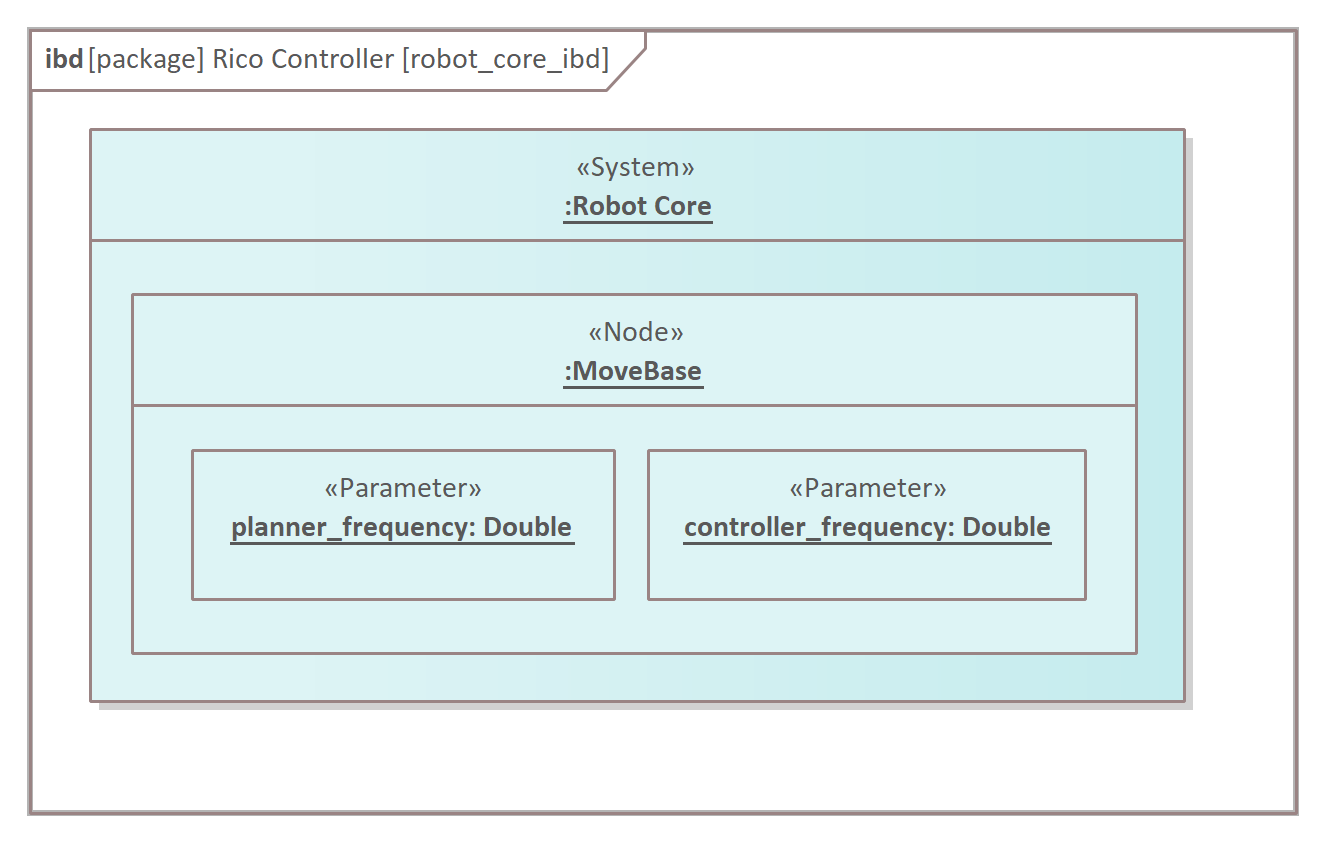
\includegraphics[scale=.85]{img/rico_pkg/robot_core_ibd.png}}
		\end{center}
		\caption{Selected elements of \stSystem{} \texttt{:Robot Core}.} 
		\label{fig:robot_core_ibd}
	\end{figure}
				
	\stCommChannel{} \texttt{:Move To to Robot Core} is depicted in Fig.~\ref{fig:move_to_2_core_cm_ibd}. It comprises three actions.
	

	\begin{figure}[H]
		\centering
		\begin{center}
			{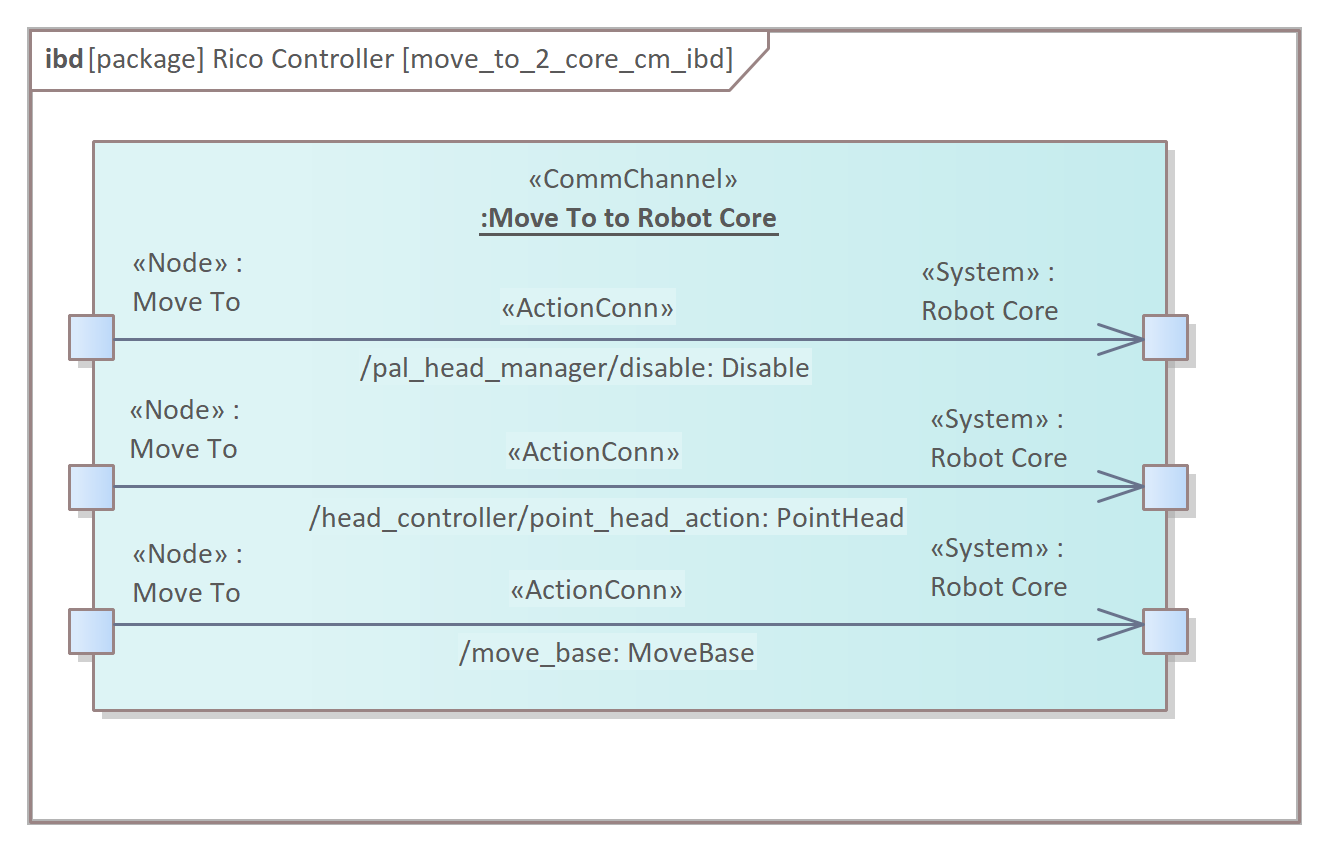
\includegraphics[scale=1.1]{img/rico_pkg/move_to_2_core_cm_ibd.png}}
		\end{center}
		\caption{Example of \stCommChannel{}.} 
		\label{fig:move_to_2_core_cm_ibd}
	\end{figure}
	
		
	The part of the scenario generally described in Fig.~\ref{fig:general_sd} is depicted in detail in Fig.~\ref{fig:motion_execution_sd}. The presentation remains conceptual from the behavioural point of view, but it considers the particular parts of the \stSystem{} \texttt{:Rico}.
	
	\begin{figure}[H]
		\centering
		\begin{center}
			{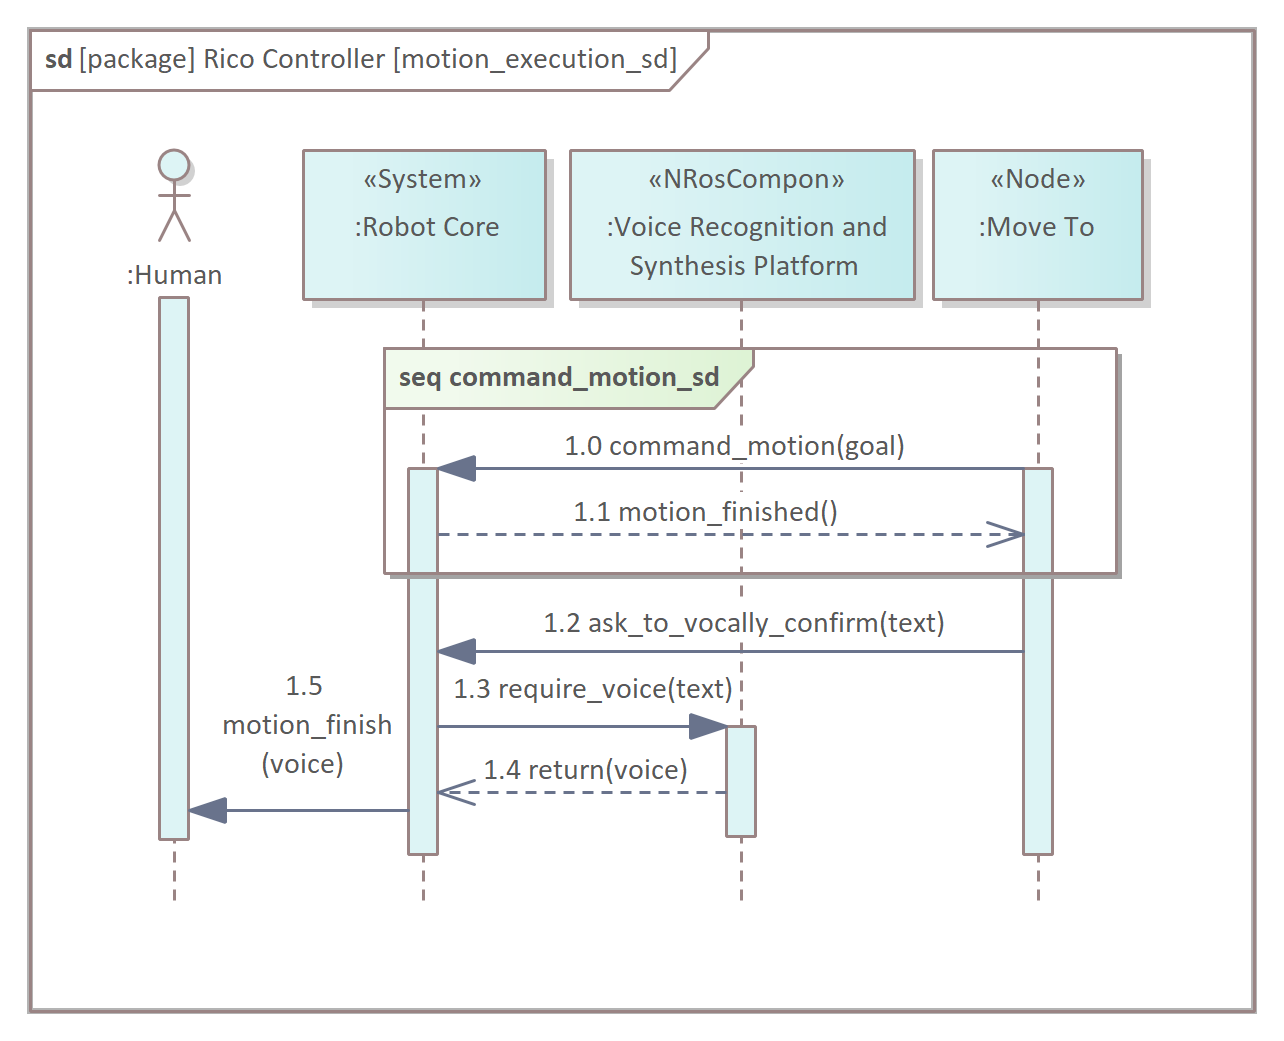
\includegraphics[scale=1.1]{img/rico_pkg/motion_execution_sd.png}}
		\end{center}
		\caption{Motion execution operation.} 
		\label{fig:motion_execution_sd}
	\end{figure}


	Finally, the particular communication methods are specified on the most detailed, ROS-specific level (Fig.~\ref{fig:command_motion_sd}). The command\_motion operation includes the sequence of four steps of communication. Three Actions realise the communication, one utilised twice. The diagram comprises extra notes that make it easier to interpret.
	
	\begin{figure}[H]
		\centering
		\begin{center}
			{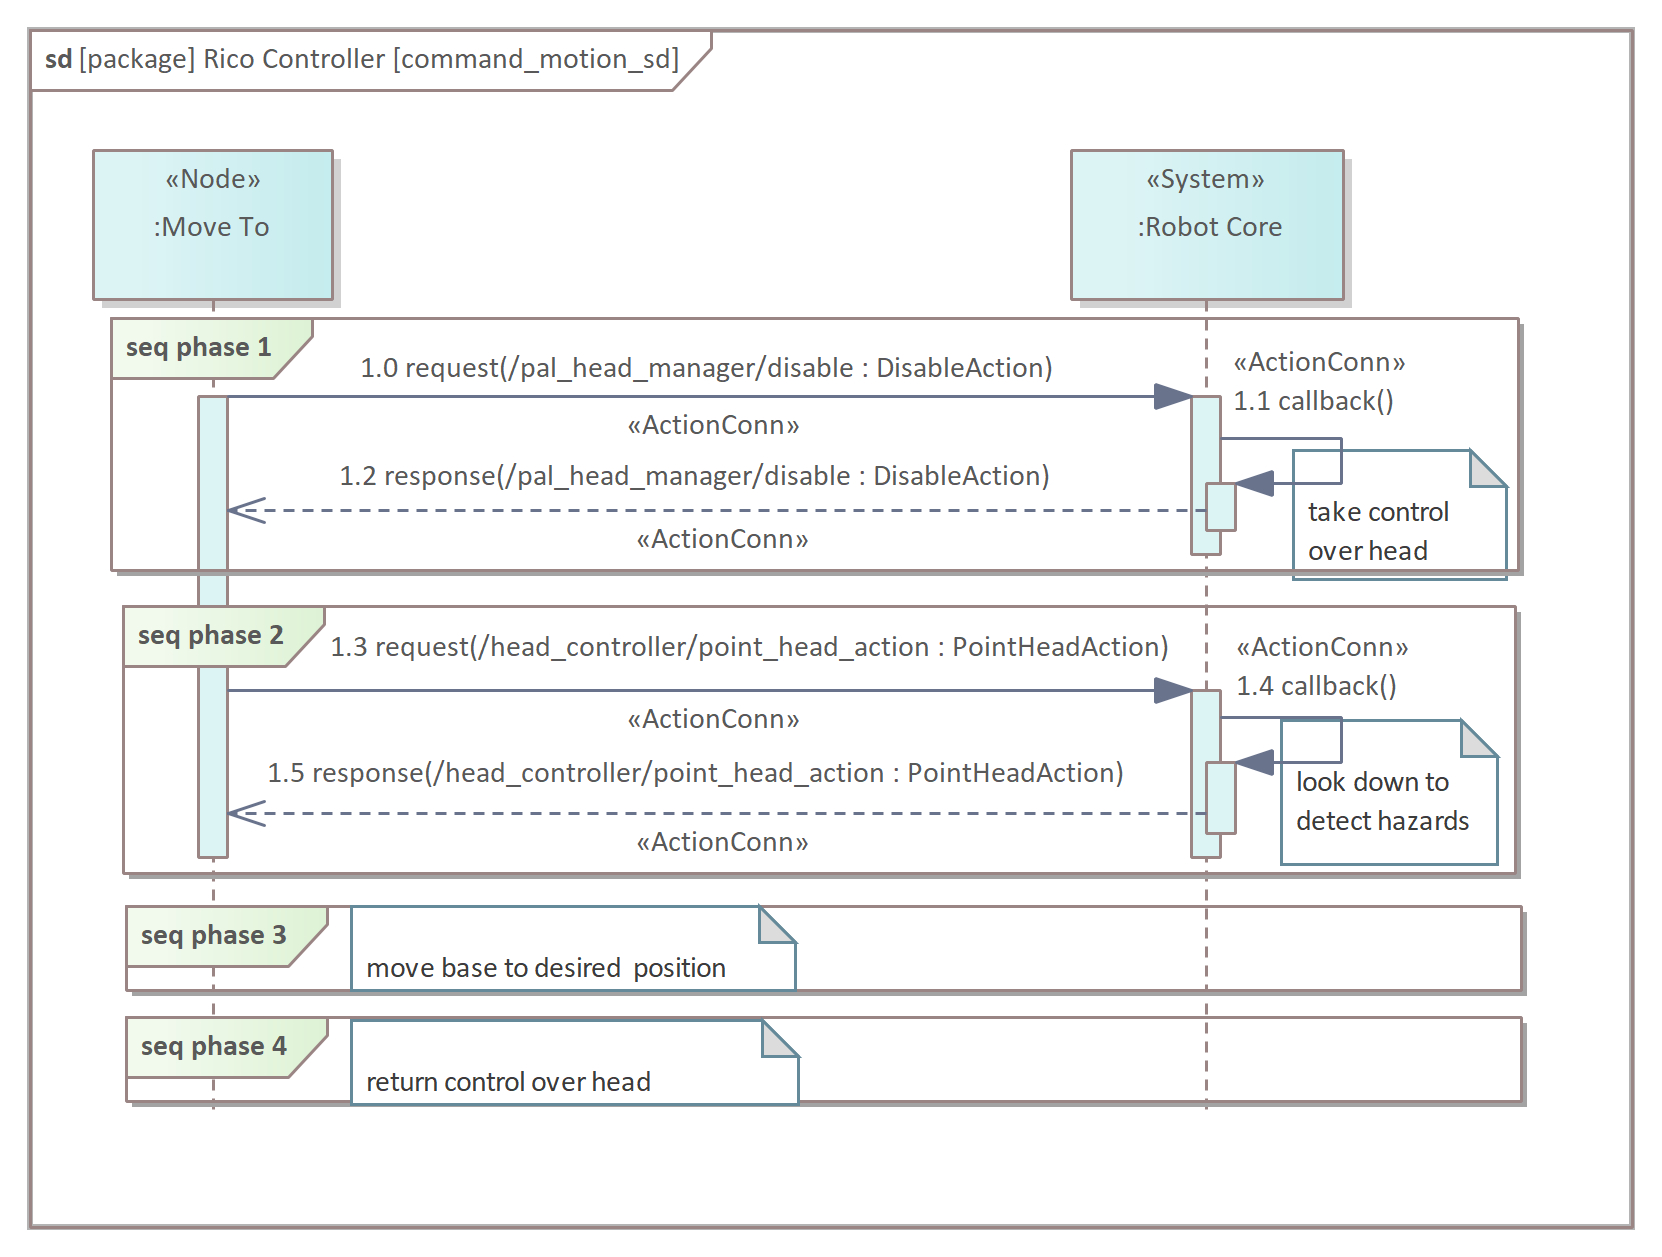
\includegraphics[scale=1.0]{img/rico_pkg/command_motion_sd.png}}
		\end{center}
		\caption{Command motion operation with detailed Communication methods presentation.} 
		\label{fig:command_motion_sd}
	\end{figure}
	
	The part of the \stWorkspace{} \texttt{:Rico} that includes previously mentioned elements is presented in Fig.~\ref{fig:rico_workspace_nodes_bdd} and Fig.~\ref{fig:rico_workspace_msgs_bdd}.
	
	\begin{figure}[H]
		\centering
		\begin{center}
			{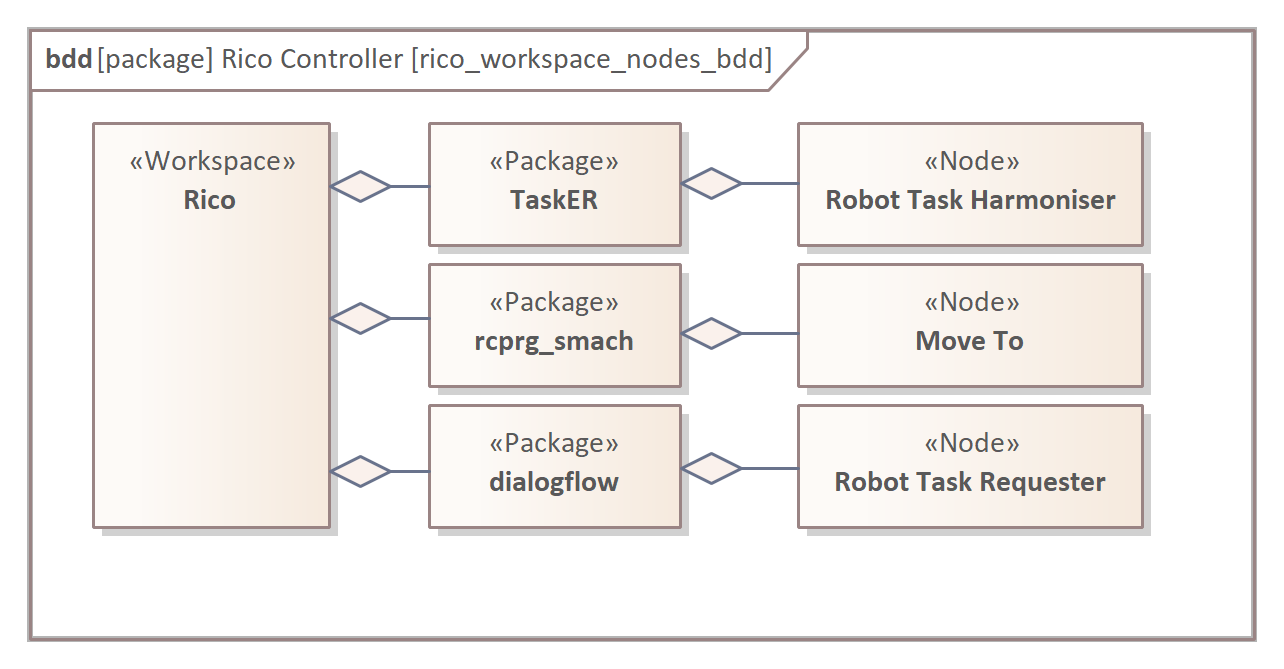
\includegraphics[scale=1.0]{img/rico_pkg/rico_workspace_nodes_bdd.png}}
		\end{center}
		\caption{Rico \stWorkspace{} composition -- Packages with Nodes.}
		\label{fig:rico_workspace_nodes_bdd}
	\end{figure}

	\begin{figure}[H]
		\centering
		\begin{center}
			{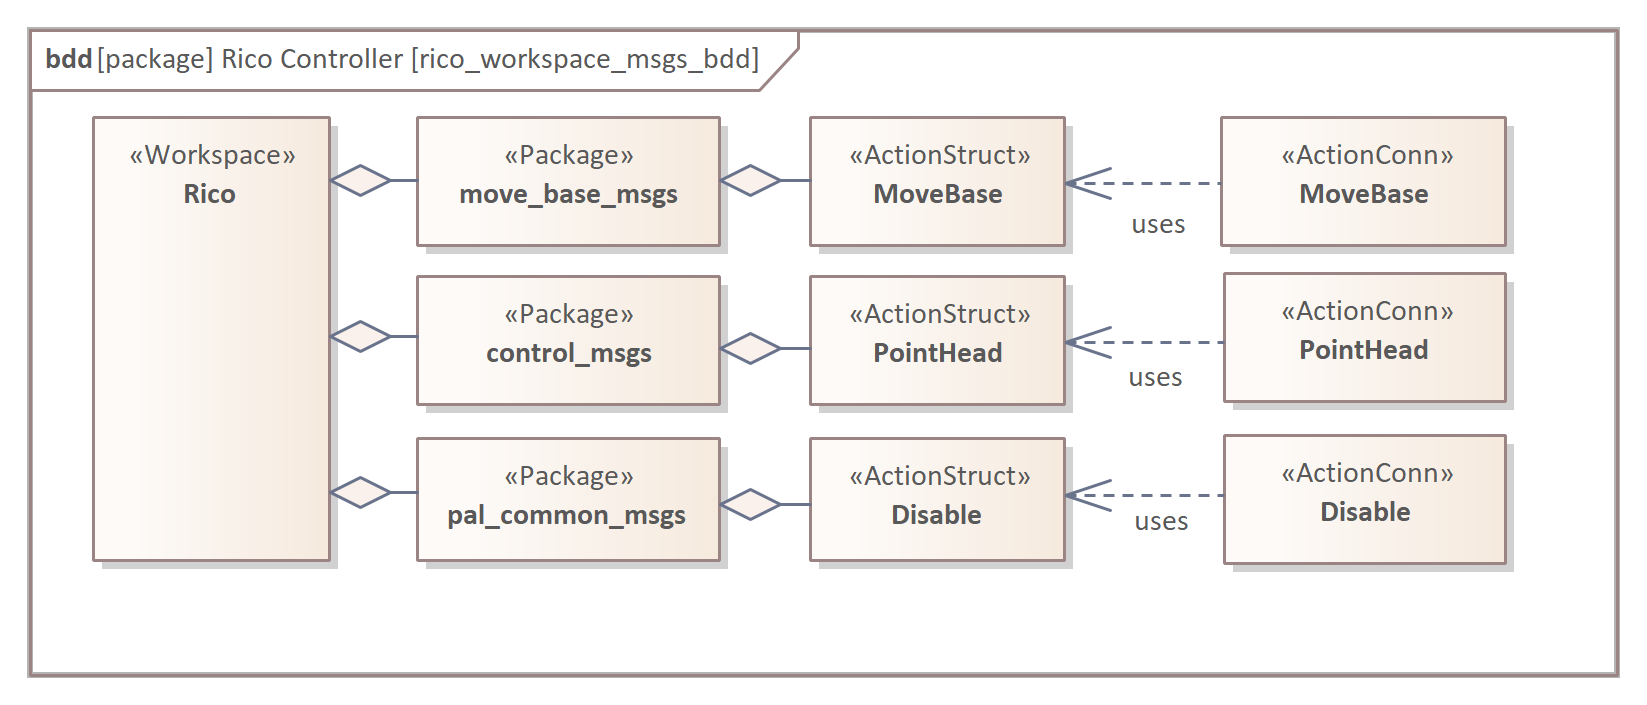
\includegraphics[scale=1.0]{img/rico_pkg/rico_workspace_msgs_bdd.png}}
		\end{center}
		\caption{Rico \stWorkspace{} composition -- Packages with Msgs.}
		\label{fig:rico_workspace_msgs_bdd}
	\end{figure}
	
			
\AtNextBibliography{\small}
\printbibliography
	
\end{document}
